%%
% This is an Overleaf template for presentations
% using the TUM Corporate Desing https://www.tum.de/cd
%
% For further details on how to use the template, take a look at our
% GitLab repository and browse through our test documents
% https://gitlab.lrz.de/latex4ei/tum-templates.
%
% The tumbeamer class is based on the beamer class.
% If you need further customization please consult the beamer class guide
% https://ctan.org/pkg/beamer.
% Additional class options are passed down to the base class.
%
% If you encounter any bugs or undesired behaviour, please raise an issue
% in our GitLab repository
% https://gitlab.lrz.de/latex4ei/tum-templates/issues
% and provide a description and minimal working example of your problem.
%%

\documentclass[
  german,            % define the document language (english, german)
  aspectratio=169,    % define the aspect ratio (169, 43)
  % handout=2on1,       % create handout with multiple slides (2on1, 4on1)
  % partpage=false,     % insert page at beginning of parts (true, false)
  % sectionpage=true,   % insert page at beginning of sections (true, false)
]{tumbeamer}


% load additional packages
\usepackage{booktabs}
\usepackage{graphicx}
\usepackage{tikz}
\usepackage{url}
\usepackage{pgfplots}
\usepackage{hyperref}
\usepackage{pmboxdraw}
\usepackage{float}
\usepackage{babel}[ngerman]
\usepackage{csquotes}[autostyle]
\usepackage[useregional]{datetime2}
\usepackage{listings}
\usepackage{xurl}
\usepackage{enumerate}
\usepackage{circuitikz}
\usepackage{csquotes}
\usepackage{tikz-timing}

%\usepackage{minted}
%\usemintedstyle{borland}
\usetikzlibrary{patterns}
\pgfplotsset{compat=1.18}

% tikz
\usetikzlibrary{overlay-beamer-styles}
\usetikzlibrary{arrows,backgrounds,positioning,shapes,,patterns,patterns.meta,matrix,arrows,shapes.geometric}
\usetikzlibrary{matrix}
% requires circuitikz >= 1.1.0
% for distros with older distributions, install TeX Live manually
% instead of using your package manager
% see: https://tug.org/texlive/quickinstall.html
\ctikzset{logic ports=european}

% minted

\lstset {
    frame=single,
    tabsize=4,
    breaklines=true,
    xleftmargin=5pt,
    xrightmargin=5pt,
    basicstyle=\ttfamily\footnotesize,
    %language=[RISC-V]Assembler,
}

\hypersetup { 
  colorlinks=true,
  urlcolor=blue,
  filecolor=black,
  linkcolor=black
}

% tikz  
\usetikzlibrary{fit}

% image path
\graphicspath{ {../resources/} }

% presentation metadata
\title{Übung 07: Sequenzielle Logik}

\subtitle{Einführung in die Rechnerarchitektur}

\author{\theAuthorName}

\institute{\theGroupName\\\theSchoolName\\\theUniversityName}
\date{2. -- \DTMdisplaydate{2024}{12}{8}{-1}}

\footline{\insertauthor~|~\insertshorttitle~|~\insertshortdate}


% macro to configure the style of the presentation
\TUMbeamersetup{
  title page = TUM tower,         % style of the title page
  part page = TUM toc,            % style of part pages
  section page = TUM toc,         % style of section pages
  content page = TUM more space,  % style of normal content pages
  tower scale = 1.0,              % scaling factor of TUM tower (if used)
  headline = TUM threeliner,      % which variation of headline to use
  footline = TUM default,         % which variation of footline to use
  % configure on which pages headlines and footlines should be printed
  headline on = {title page},
  footline on = {every page, title page=false},
}


% available frame styles for title page, part page, and section page:
% TUM default, TUM tower, TUM centered,
% TUM blue default, TUM blue tower, TUM blue centered,
% TUM shaded default, TUM shaded tower, TUM shaded centered,
% TUM flags
%
% additional frame styles for part page and section page:
% TUM toc
%
% available frame styles for content pages:
% TUM default, TUM more space
%
% available headline options:
% TUM empty, TUM oneliner, TUM twoliner, TUM threeliner, TUM logothreeliner
%
% available footline options:
% TUM empty, TUM default, TUM infoline

\begin{document}

\maketitle

\begin{frame}[c]{Mitschriften \& Infos}{}
  \begin{minipage}[t]{\textwidth}
    \begin{columns}[c]
      \begin{column}{0.8\textwidth}
        Montags: \href{\zulipMo}{\zulipMo}
      \end{column}
      \begin{column}{0.2\textwidth}
        \includegraphics[width=0.8\linewidth]{\zulipMoQrFilename}
      \end{column}
    \end{columns}
  \end{minipage}
  \rule{\textwidth}{0.4pt}
  \begin{minipage}[t]{\textwidth}
    \begin{columns}[c]
      \begin{column}{0.8\textwidth}
        Donnerstags: \href{\zulipDo}{\zulipDo}
      \end{column}
      \begin{column}{0.2\textwidth}
        \includegraphics[width=0.8\linewidth]{\zulipDoQrFilename}
      \end{column}
    \end{columns}
  \end{minipage}
  \ifdefined\myWebsite
  \rule{\textwidth}{0.4pt}
  \centering
  Website: \href{\myWebsite}{\myWebsite}
  \fi
\end{frame}

\begin{frame}[c]{}{}
  \begin{center}
    \LARGE  Keine Garantie für die Richtigkeit der Tutorfolien.

    \Large Bei Unklarheiten/Unstimmigkeiten haben VL/ZÜ-Folien recht!
  \end{center}
\end{frame}

\begin{frame}[c]{Inhaltsübersicht}{}
  \begin{columns}[c]
    \begin{column}{1\textwidth}
      \begin{itemize}
        \item Quiz
        \item Wiederholung
        \item Tutorblatt
        \begin{itemize}
          \item Wellenformen
          \item Program Counter
          \item Linear-Rückgekoppeltes-Schieberegister
        \end{itemize}
      \end{itemize}
    \end{column}
  \end{columns}
\end{frame}

\begin{frame}[c, fragile]{}{}
  \begin{center}
    \vspace{0.5cm}
    \begin{block}{Zitat der Woche}
      \vspace{0.5cm}
      \begin{quote}
        ``Nach 60 Jahren wo ich diese blöde Vorlesung hier halte''
        \vspace{0.5cm}
        \flushright{\textbf{- Prof. Dr. Robert Wille (geboren 11.11.1982)}}
      \end{quote}
      \vspace{0.5cm}
    \end{block}
    \vspace{0.5cm}
    Quelle: \href{https://tum.live/w/ws24EidR/50022?t=5533}{Lecture: November 19. 2024 (tum.live)}
\end{center}
\end{frame}

\begin{frame}[fragile, c]{Sequentielle Schaltungen}
	\begin{columns}[c]
		\begin{column}{0.6\textwidth}
			\begin{itemize}
				\item \textbf{kombinatorische} Schaltungen: zustandsfrei, Ausgänge nur abhängig von Eingängen. \\ $\rightarrow$ z.B.: HA letzte Woche, Addierer, XOR, $\ldots$
				\item \textbf{sequentielle} Schaltungen: zustandsbehaftet, Ausgänge wirken über Rückkopplung auf Schaltung ein! (Zyklus im Graphen)\\ $\rightarrow$ z.B.: Zähler, Speicher, Statusautomaten, %$\ldots$
				\item sequentielle Schaltungen ermöglichen es erst, komplexe Dinge wie Prozessoren zu bauen!
				      %\item Multiplexer: Leitet Eingang abhängig von Steuersignal durch
				      %\item ALU (arithmetic logic unit): Recheneinheit eines Prozessors
				      %\item Latches: Speichereinheit für 1 Bit
				      %\item Flip-Flops: Taktflankengesteuertes Latch
				      %\item D-Latch: Data-Eingang und Enable-Eingang
			\end{itemize}
		\end{column}
		\begin{column}{0.4\textwidth}
			\begin{center}
				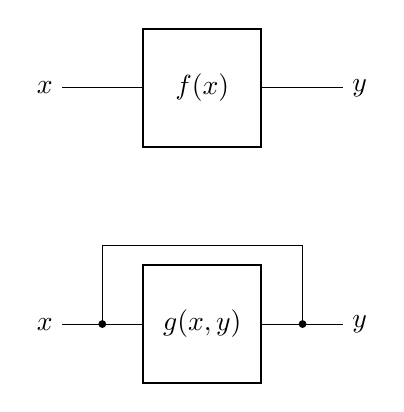
\begin{tikzpicture}[comp/.style={rectangle, draw=black, thick, minimum size=1.5cm}]
					\node[comp] (n1) {$f(x)$};
					\node[left of=n1, xshift = -1cm] (n1l) {$x$};
					\node[right of=n1, xshift = 1cm] (n1r) {$y$};
					\draw (n1l) -- (n1.west);
					\draw (n1.east) -- (n1r);

					\node[comp] (n2) [below of=n1, yshift=-2cm] {$g(x, y)$};
					\node[left of=n2, xshift=-1cm] (n2l) {$x$};
					\node[right of=n2, xshift=1cm] (n2r) {$y$};

					\draw (n2l) -- (n2.west) node[midway, fill=black, circle, inner sep=1pt] (n2ml) {};
					\draw (n2.east) -- (n2r) node[midway, fill=black, circle, inner sep=1pt] (n2mr) {};

					\node[above of=n2ml] (n2lu) {};
					\node[above of=n2mr] (n2ru) {};
					\draw (n2ml.center) -| (n2lu.center);
					\draw (n2mr.center) -- (n2ru.center);
					\draw (n2lu.center) -- (n2ru.center);
				\end{tikzpicture}
			\end{center}
		\end{column}
	\end{columns}
\end{frame}

\begin{frame}[c]{RS-Latch}{}
	\begin{columns}[c]
		\begin{column}{0.5\textwidth}
			\centering
			
\includegraphics[width=0.9\textwidth]{w07_RS_Flip-flop_(NOR).svg.png}
		\end{column}
		\begin{column}{0.5\textwidth}
			\centering
			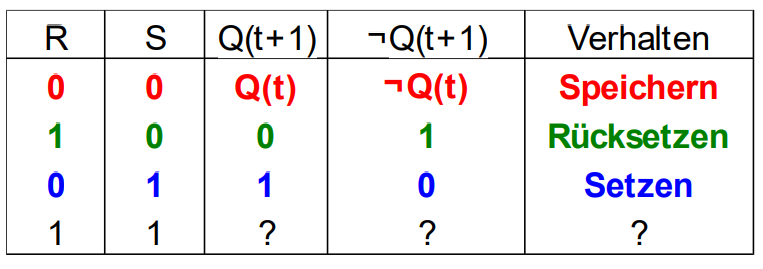
\includegraphics[width=0.9\textwidth]{w07_rs_table_lv.png}
		\end{column}
	\end{columns}
\end{frame}

\begin{frame}[c]{Latches}{}
	\begin{columns}[c]
		\begin{column}{0.5\textwidth}
			\centering  \textbf{NOR-SR-Latch}\\
			\vspace{0.3cm}
			\begin{itemize}
				\item  pegelgesteuert
				\item \textbf{S}et, \textbf{R}eset
				\item \enquote{verbotener} Zustand $(1,1) \implies Q = \neg Q = 0$
			\end{itemize}
			\vspace{0.3cm}
			\begin{center}
				\begin{circuitikz}
					\node[flipflop SR] (sr) {};
					\node[right of=sr, xshift=2cm] (arr) {$
							\begin{array}{|c|c|c|}
								\hline
								S & R & Q                 \\
								\hline
								0 & 0 & Q_{\textrm{prev}} \\
								0 & 1 & 0                 \\
								1 & 0 & 1                 \\
								1 & 1 & 0                 \\
								\hline
							\end{array}
						$};
				\end{circuitikz} 
			\end{center}
		\end{column}
		\begin{column}{0.5\textwidth}
			\centering  \textbf{NAND-SR-Latch}\\
			\vspace{0.3cm}
			\begin{itemize}
				\item  pegelgesteuert
				\item $\neg S, \neg R$
				\item \enquote{verbotener} Zustand $(0,0) \implies Q = \neg Q = 1$
			\end{itemize}
			\vspace{0.3cm}
			\begin{center}
				\begin{circuitikz}
					\node[flipflop SR] (sr) {};
					\node[right of=sr, xshift=2cm] (arr) {$
							\begin{array}{|c|c|c|}
								\hline
								S & R & Q                 \\
								\hline
								0 & 0 & 1                 \\
								0 & 1 & 1                 \\
								1 & 0 & 0                 \\
								1 & 1 & Q_{\textrm{prev}} \\
								\hline
							\end{array}
						$};
				\end{circuitikz} 
			\end{center}
		\end{column}
	\end{columns}
\end{frame}

\begin{frame}[c]{Latches und Flipflops}{}
	\begin{columns}[c]
		\begin{column}{0.5\textwidth}
			\centering \textbf{D-Latch}\\
			\vspace{0.3cm}
			\begin{itemize}
				\item  pulsgesteuert
				\item transparent, wenn Schreibsignal aktiv ist
				\item Bei $E=0$ bleibt Zustand gespeichert, sonst wird $D$ übernommen.
			\end{itemize}
			\vspace{0.5cm}
			\begin{center}
				\begin{circuitikz}
					\node[flipflop D] (dff) {};
					\node[right of=dff, xshift=2cm] (arr) {
						$
							\begin{array}{|c|c|c|}
								\hline
								E             & D & Q                 \\
								\hline
								0 & 0 & Q_{\textrm{prev}} \\
								0 & 1 & Q_{\textrm{prev}} \\
								1 & 0 & 0                 \\
								1 & 1 & 1                 \\
								\hline
							\end{array}
						$};
				\end{circuitikz}
			\end{center}
		\end{column}
		\begin{column}{0.5\textwidth}
			\centering \textbf{D-Flipflop}\\
			\vspace{0.3cm}
			\begin{itemize}
				\item  taktflankengesteuert
				\item Bei fallender Flanke bleibt Zustand gespeichert, bei steigender
				      Flanke wird $D$ übernommen.
			\end{itemize}
			\vspace{0.5cm}
			\begin{center}
				\begin{circuitikz}
					\node[flipflop D] (dff) {};
					\node[right of=dff, xshift=2cm] (arr) {
						$
							\begin{array}{|c|c|c|}
								\hline
								CLK             & D & Q                 \\
								\hline
								\texttiming{HL} & 0 & Q_{\textrm{prev}} \\
								\texttiming{HL} & 1 & Q_{\textrm{prev}} \\
								\texttiming{LH} & 0 & 0                 \\
								\texttiming{LH} & 1 & 1                 \\
								\hline
							\end{array}
						$};
				\end{circuitikz}
			\end{center}
		\end{column}
	\end{columns}
\end{frame}

\begin{frame}[c]{ALU}{}
	\begin{columns}[c]
		\begin{column}{0.5\textwidth}
			\begin{itemize}
				\item \textbf{A}rithmetic \textbf{L}ogic \textbf{U}nit zur Berechnung von arithmetischen und logischen Basisoperationen
				\item n-Bit-ALU mit:
				 \begin{itemize}
          \item zwei n-Bit-Operanden a, b, Eingangscarry c
          \item m-Bit select-Eingang, der auswählt, welche Funktion ausgeführt wird
          \item (n+1)-Bit-Ausgang
         \end{itemize}
			\end{itemize}
		
		\end{column}
		\begin{column}{0.5\textwidth}
			\begin{center}
				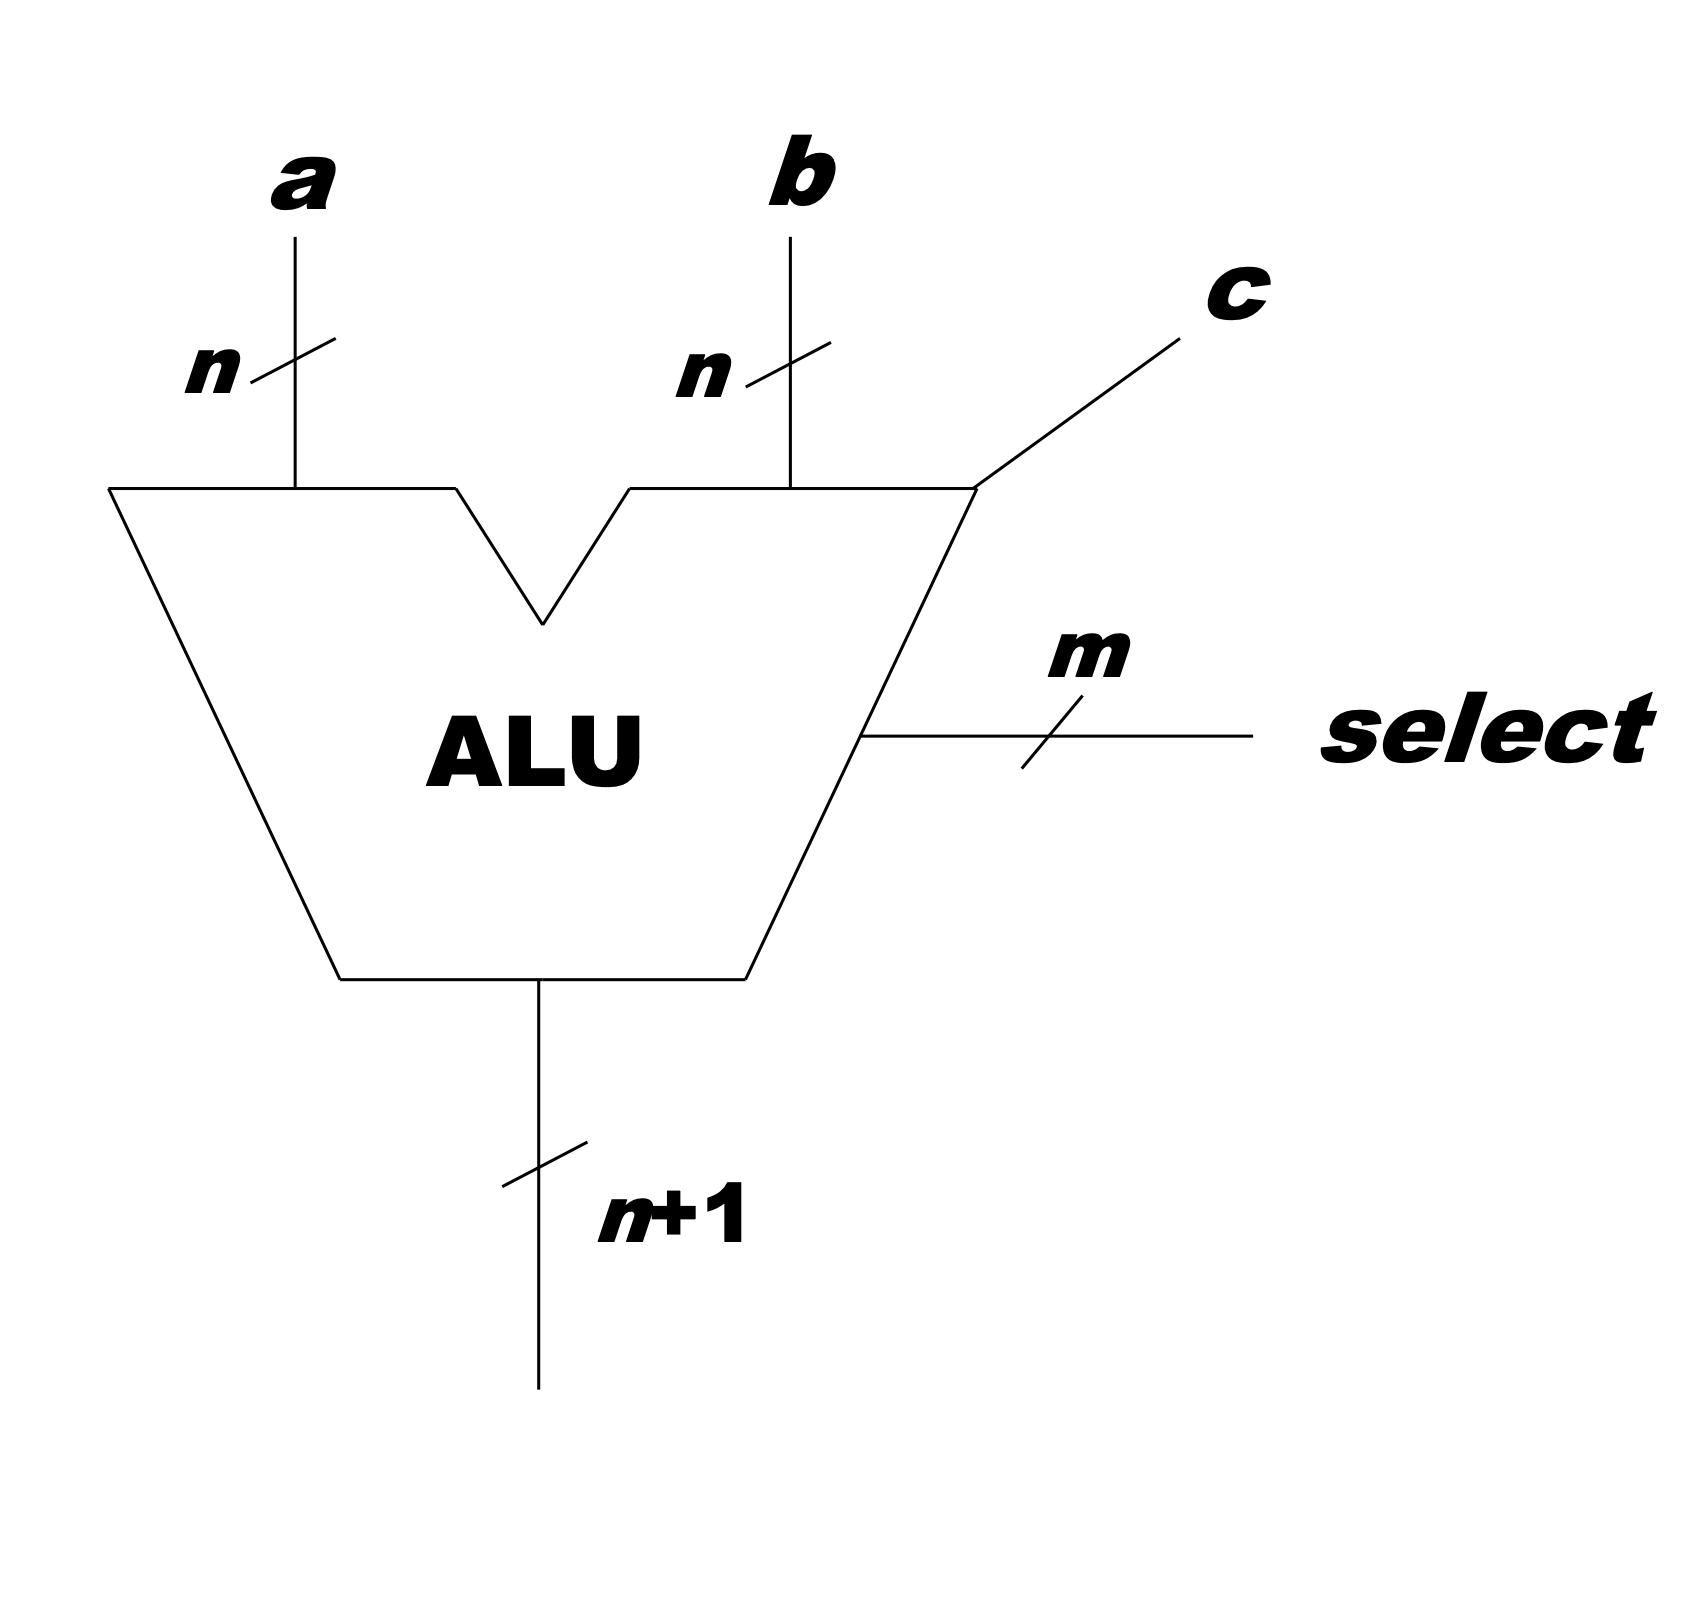
\includegraphics[width=0.8\textwidth]{w07_alu_schaltzeichen.png}
			\end{center}
		\end{column}
	\end{columns}
\end{frame}

\begin{frame}[c]{Floating-Point-Zahlen}
	\begin{itemize}
		\item Fließkommazahlen der Form $(-1)^{\textrm{sign}}\cdot 1.\textrm{mantissa}\cdot 2^{\textrm{exp}-\textrm{bias}}$
	\end{itemize}
	\begin{center}
		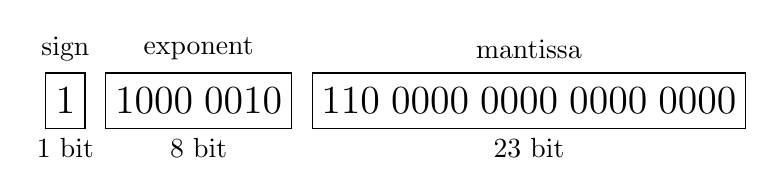
\begin{tikzpicture}
			\matrix[matrix of nodes, ampersand replacement=\&, nodes={draw, minimum width=0.5cm, minimum height=0.7cm, anchor=center}, column sep=0.25cm, font={\Large}] (mat) {
				{$1$} \& {$1000\;0010$} \& {$110\;0000\;0000\;0000\;0000$} \\
			};
			\node[above=0.3cm of mat-1-1.north, anchor=center] {\textrm{sign}};
			\node[above=0.3cm of mat-1-2.north, anchor=center] {\textrm{exponent}};
			\node[above=0.3cm of mat-1-3.north, anchor=center] {\textrm{mantissa}};

			\node[below=0cm of mat-1-1.south, anchor=north] {\textrm{1 bit}};
			\node[below=0cm of mat-1-2.south, anchor=north] {\textrm{8 bit}};
			\node[below=0cm of mat-1-3.south, anchor=north] {\textrm{23 bit}};
		\end{tikzpicture}
	\end{center}
	\begin{itemize}
		\item Bei 32-Bit-Floats: 1 Bit Vorzeichen, 8 Bit Exponent, 23 Bit Mantisse, Bias 127
		\item implizite 1 vor der Mantisse wird nicht mitgespeichert
		\item Sonderfälle $\pm0$, $\pm\infty$, $\textrm{NaN}$: nicht relevant für HA
		\item Visualisierung: \href{https://evanw.github.io/float-toy/}{Float Toy}
	\end{itemize}
\end{frame}

\begin{frame}[c]{Floating-Point-Zahlen: Beispiel}
	\begin{center}
		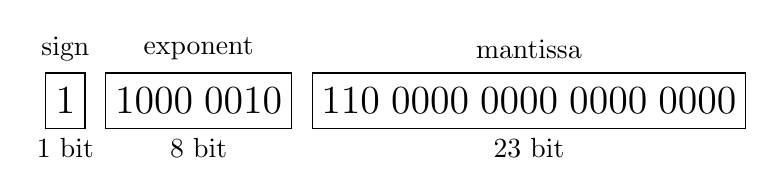
\begin{tikzpicture}
			\matrix[matrix of nodes, ampersand replacement=\&, nodes={draw, minimum width=0.5cm, minimum height=0.7cm, anchor=center}, column sep=0.25cm, font={\Large}] (mat) {
				{$1$} \& {$1000\;0010$} \& {$110\;0000\;0000\;0000\;0000$} \\
			};
			\node[above=0.3cm of mat-1-1.north, anchor=center] {\textrm{sign}};
			\node[above=0.3cm of mat-1-2.north, anchor=center] {\textrm{exponent}};
			\node[above=0.3cm of mat-1-3.north, anchor=center] {\textrm{mantissa}};

			\node[below=0cm of mat-1-1.south, anchor=north] {\textrm{1 bit}};
			\node[below=0cm of mat-1-2.south, anchor=north] {\textrm{8 bit}};
			\node[below=0cm of mat-1-3.south, anchor=north] {\textrm{23 bit}};
		\end{tikzpicture}
		\vspace{0.3cm}
		\begin{enumerate}
			\item Vorzeichen: $(1)_2 \rightarrow (-1)$
			\item Exponent: $(1000\;0010)_2 = 130$, $130-\textrm{bias} = 130-127 = 3$
			\item Mantisse: $(1.110\;0000\;0000\;0000\;0000)_2 = 1.75$
		\end{enumerate}
		\vspace{0.3cm}
		\Large
		\[
			n = (-1) \cdot 1.75 \cdot 2^3 = -14
		\]
	\end{center}
\end{frame}

\begin{frame}[c]{}{} 
  \begin{center}
    \LARGE Fragen?
  \end{center}
  \vspace{0.5cm}
  \begin{center}
    \LARGE Bis zum nächsten Mal ;) \\
  \end{center}
  \vspace{1.0cm}
  \begin{center}
    \small Folien inspiriert von Niklas Ladurner und Prof. Dr. Robert Wille
  \end{center}
\end{frame}

\end{document}